\documentclass[journal,12pt,twocolumn]{IEEEtran}
\usepackage{graphicx}
\graphicspath{{./images/}}
\usepackage{amsmath,amssymb,amsfonts,amsthm}
\newcommand{\myvec}[1]{\ensuremath{\begin{pmatrix}#1\end{pmatrix}}}
\usepackage{listings}
\usepackage{watermark}
\usepackage{titlesec}
\let\vec\mathbf
\lstset{
frame=single, 
breaklines=true,
columns=fullflexible
}
\thiswatermark{\centering \put(0,-105.0){
\includegraphics[scale=0.2]{logo2.png}} }
\title{\mytitle}
\title
{
Matrix Assignment - Circle
}
\author{Surajit Sarkar}
\begin{document}
\maketitle
\tableofcontents
\bigskip


\section{\textbf{Problem}}
Let P ($a\sec \theta,b \tan \theta$) and Q ($a\sec \phi,b\tan\phi$),where $\theta+\phi={\frac{\pi}{2}}$,be two points on the hyperbola $\frac{x^2}{a^2}-\frac{y^2}{b^2}=1$.if (h,k) is the point pf intersection of normals at P and Q,then k is equal to


\section{\textbf{solution}}

Equation of normal at Q for a conic
\begin{equation}
{\vec{{x}}^T{\vec V}{\vec x}+2{\vec u}^T{\vec x}}+f=0
\end{equation}
where
\begin{equation}
    \vec n=\vec {V_q+u}
\end{equation}
\begin{equation}
    \vec m=\vec R_{\frac{\pi}{2}}\vec n
\end{equation}
\begin{equation}
    \vec m^T\myvec{\vec {x-q}}=0
\end{equation}
normal at 
\begin{equation}
  \vec{  k = q}
\end{equation}
For $L_1$
\begin{equation}
    \vec m^T_1\myvec{\vec x-\vec q_1}=0
\end{equation}
\\
For $L_2$
\begin{equation}
    \vec m^T_2\myvec{\vec x-\vec q_2}=0
\end{equation}
Point of intersection
\begin{equation}
    \myvec{\vec {m}_1 &\vec {m}_2} \vec R=\myvec{\vec m_1 & \vec q_1 \\ \vec m_2 & \vec q_2 }
\end{equation}
\\
\begin{equation}
    \vec R =\vec m^{-1} \myvec{\vec m^T_1 & \vec q_1 \\ \vec m^T_2 & \vec q_2 }
\end{equation}
Using python we get the value of k
\begin{equation}
    \vec k=-\myvec{\frac{a^2+b^2}{b}}
\end{equation}
\begin{lstlisting}
https://github.com/sssurajit/fwc/blob/main/matrix/conics/codes/sconic.py
\end{lstlisting}
\section{\textbf{Figure}}

    \centering
    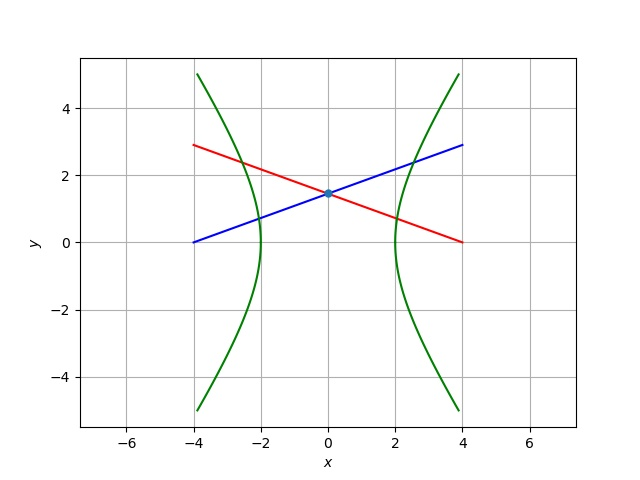
\includegraphics[width=\columnwidth]{fig.jpg}
    \label{fig:my_label}
    
\section{\textbf{Code Link}}

\begin{lstlisting}
https://github.com/sssurajit/fwc/blob/main/matrix/conics/codes/conic.py
\end{lstlisting}
Execute the code by using the command
\\ \textbf{python3 conic.py}

\end{document}

